% $Id: template.tex 11 2007-04-03 22:25:53Z jpeltier $

\documentclass{vgtc}                          % final (conference style)
%\documentclass[review]{vgtc}                 % review
%\documentclass[widereview]{vgtc}             % wide-spaced review
%\documentclass[preprint]{vgtc}               % preprint
%\documentclass[electronic]{vgtc}             % electronic version

%% Uncomment one of the lines above depending on where your paper is
%% in the conference process. ``review'' and ``widereview'' are for review
%% submission, ``preprint'' is for pre-publication, and the final version
%% doesn't use a specific qualifier. Further, ``electronic'' includes
%% hyperreferences for more convenient online viewing.

%% Please use one of the ``review'' options in combination with the
%% assigned online id (see below) ONLY if your paper uses a double blind
%% review process. Some conferences, like IEEE Vis and InfoVis, have NOT
%% in the past.

%% Figures should be in CMYK or Grey scale format, otherwise, colour 
%% shifting may occur during the printing process.

%% These few lines make a distinction between latex and pdflatex calls and they
%% bring in essential packages for graphics and font handling.
%% Note that due to the \DeclareGraphicsExtensions{} call it is no longer necessary
%% to provide the the path and extension of a graphics file:
%% \includegraphics{diamondrule} is completely sufficient.
%%
\ifpdf%                                % if we use pdflatex
  \pdfoutput=1\relax                   % create PDFs from pdfLaTeX
  \pdfcompresslevel=9                  % PDF Compression
  \pdfoptionpdfminorversion=7          % create PDF 1.7
  \ExecuteOptions{pdftex}
  \usepackage{graphicx}                % allow us to embed graphics files
  \DeclareGraphicsExtensions{.pdf,.png,.jpg,.jpeg} % for pdflatex we expect .pdf, .png, or .jpg files
\else%                                 % else we use pure latex
  \ExecuteOptions{dvips}
  \usepackage{graphicx}                % allow us to embed graphics files
  \DeclareGraphicsExtensions{.eps}     % for pure latex we expect eps files
\fi%

%% it is recomended to use ``\autoref{sec:bla}'' instead of ``Fig.~\ref{sec:bla}''
\graphicspath{{figures/}{pictures/}{images/}{./}} % where to search for the images

\usepackage{microtype}                 % use micro-typography (slightly more compact, better to read)
\PassOptionsToPackage{warn}{textcomp}  % to address font issues with \textrightarrow
\usepackage{textcomp}                  % use better special symbols
\usepackage{mathptmx}                  % use matching math font
\usepackage{times}                     % we use Times as the main font
\renewcommand*\ttdefault{txtt}         % a nicer typewriter font
\usepackage{cite}                      % needed to automatically sort the references
\usepackage{tabu}                      % only used for the table example
\usepackage{booktabs}                  % only used for the table example
%% We encourage the use of mathptmx for consistent usage of times font
%% throughout the proceedings. However, if you encounter conflicts
%% with other math-related packages, you may want to disable it.


%% If you are submitting a paper to a conference for review with a double
%% blind reviewing process, please replace the value ``0'' below with your
%% OnlineID. Otherwise, you may safely leave it at ``0''.
\onlineid{0}

%% declare the category of your paper, only shown in review mode
\vgtccategory{Research}

%% allow for this line if you want the electronic option to work properly
\vgtcinsertpkg

%% In preprint mode you may define your own headline.
%\preprinttext{To appear in an IEEE VGTC sponsored conference.}

%% Paper title.

\title{Design study project: Suicide Rates}

%% Author and Affiliation (multiple authors with single affiliations).
\author{Christian Rauch\thanks{e-mail: a01202875@unet.univie.ac.at} %
\and Daniel Hanzer\thanks{e-mail: a01349699@unet.univie.ac.at} %
\and Roman Schneglberger\thanks{e-mail: a01127050@unet.univie.ac.at}}
\affiliation{\scriptsize University of Vienna \\ Faculty of Computer Science}

%%%%%%%%%%%%%%%%%%%%%%%%%%%%%%%%%%%%%%%%%%%%%%%%%%%%%%%%%%%%%%%%
%%%%%%%%%%%%%%%%%%%%%% START OF THE PAPER %%%%%%%%%%%%%%%%%%%%%%
%%%%%%%%%%%%%%%%%%%%%%%%%%%%%%%%%%%%%%%%%%%%%%%%%%%%%%%%%%%%%%%%%

\begin{document}

\maketitle

\section{Motivation}

\subsection{Background information}

Our Application deals with the suicide rate of a total of 41 countries. The goal of this project was to create a visualization that show a variety of graphs that are changeable by user interactions. The graphs are able to filter to get more precisely data out of it. It is possible to compare different countries with each other. Furthermore, it is possible to compare the suicide rates with unemployment rates, poverty rates as well as Gross domestic product (gdp) rates for each country. These comparisons should help to find possible parallel between the data in order to find any conclusions about the reasons for suicidal ones. 

\subsection{Tasks}

Our tasks was to visualize the existing records as good as possible. One of our tasks was creating a heatmap. In addition, a timeline should be available to filter for certain periods of time. In general, our the main task was to install meaningful filters or groupings to give the graphs as much meaning as possible. Another task was to find an explanation for the reason for the increased suicide rates in certain countries or regions, therefore we compared them with gdp, unemployment and poverty rates and visualized these through a matrix scatterplot and a line chart over time. Another task was comparing different countries or regions with one another over certain years. 

\subsection{Users}

On the one hand, our users are generally interested in our project, as well as users who conduct research in the field of suicide. Our users should be able to better understand the records by filtering them. For example, users might question why certain countries have a higher suicide rate than others and whether it involves economic or geographic causes. In particular, the course of suicide rates over time are relevant for this. Potential users may include journalists, researchers and psychologists.

\subsection{Data}

The Project focused mainly on the Dataset "Suicide rates" from OECD Data. The Data are from the year 1960 until to the year 2015 and include the amount of suicides per 100.000 in percentage. Altogether, the data of 41 countries are presented in this dataset. Furthermore, we used "Gross domestic product (GDP)", "Poverty rate", as well as "Unemployment rate" from OECD Data for comparing these datasets with the suicide rates.  The Data from GDP are from the year 1960 until to the year 2015 and include 40 countries. The Data from Poverty rate are from the year 1976 until to the year 2015 and include 40 countries. The Data from Unemployment rate are from the year 1953 until to the year 2015 and include 40 countries. One problem with our Data was to merge them together. Another one was that not for each country are Data available for each year, so to speak there are a lot of null values in the existing records.


\section{Related work}

\subsection{Other visualizations we discovered during this project:}

We did a lot of research in advance on interesting large datasets. From data visualisation point of view(Figure \ref{fig:tableau}) and also in scientific papers (Figure \ref{fig:scientific}), which deal with the topic, as these also contain graphics to clarify the text/make a point. These papers had mostly poor graphics included, or tables with numerical values. There were also some visualizations on Tableau-Public - these showed small details of the total amount of data. For example only for a few countries, not linking the the data to other datasets or providing interactivity. OECD(Figure \ref{fig:oecd}) website shows also graphs with their information. The solution can be used on many visualization topics.

\begin{figure}[tb]
\centering
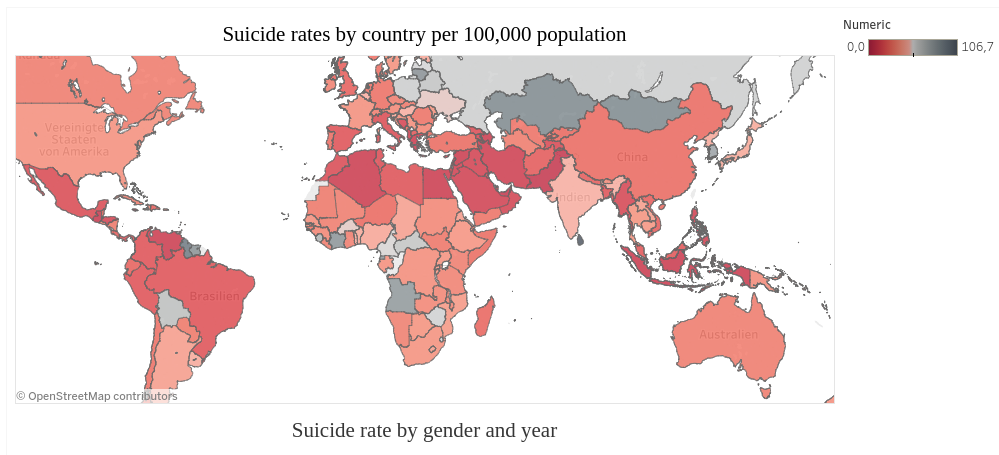
\includegraphics[width=\columnwidth]{image/roman/researches.png}
\caption{Vis from Tableau}
\label{fig:tableau} 
\end{figure}

\begin{figure}[tb]
\centering
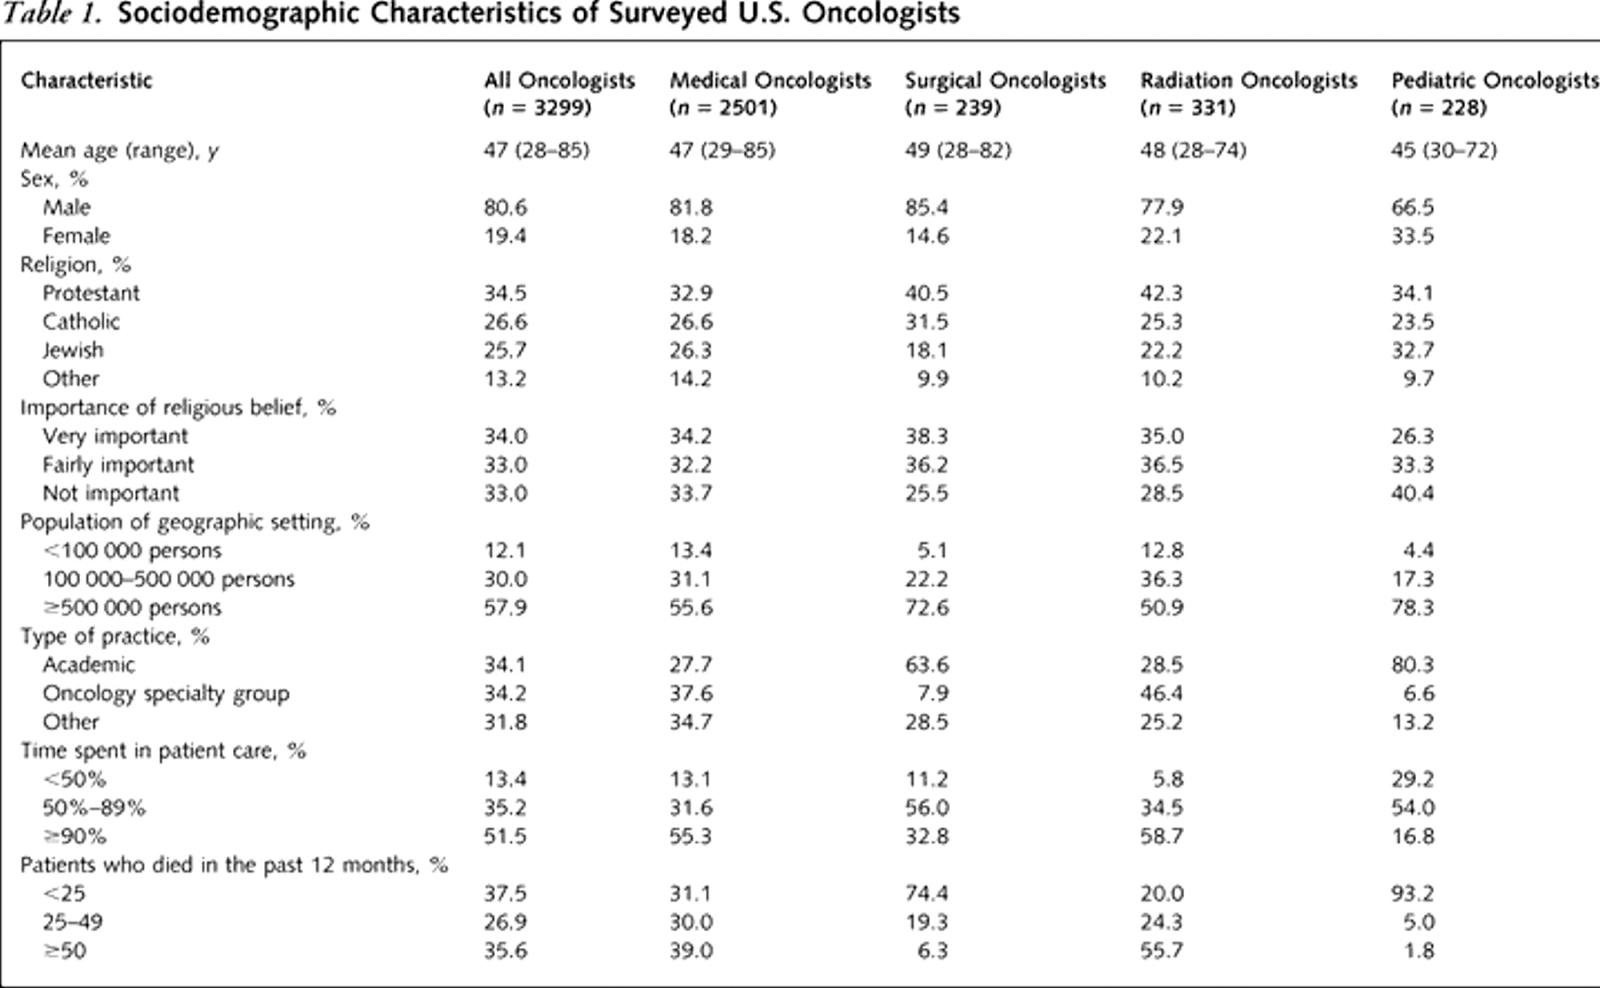
\includegraphics[width=\columnwidth]{image/roman/scientificvalues.png}
\caption{Data usage in scientific papers}
\label{fig:scientific} 
\end{figure}

\begin{figure}[tb]
\centering
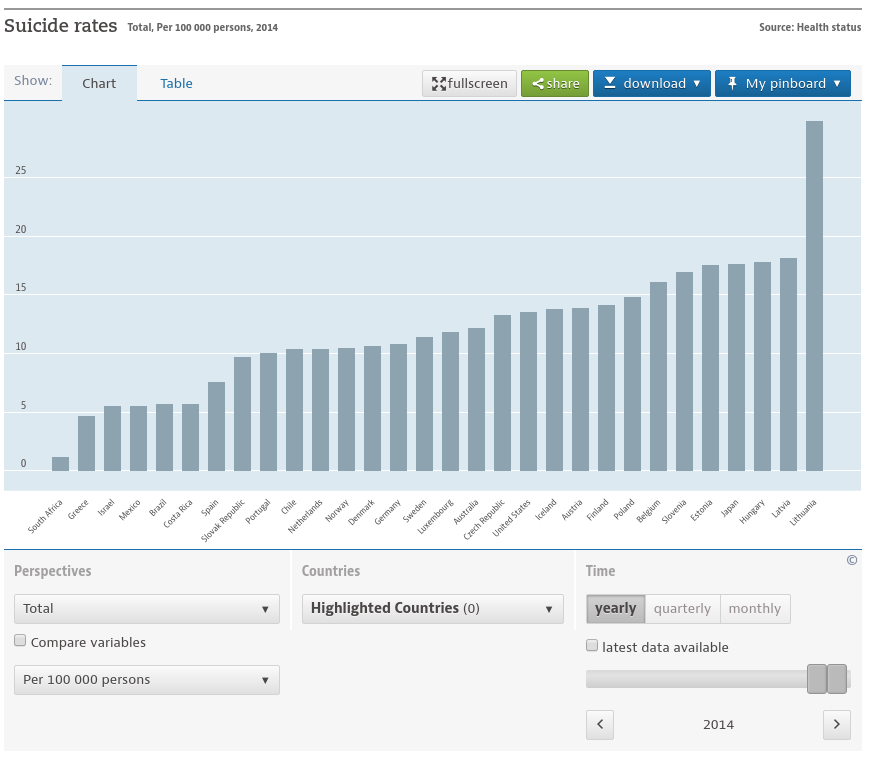
\includegraphics[width=\columnwidth]{image/roman/oecd.png}
\caption{View from oecd webpage}
\label{fig:oecd} 
\end{figure}

\subsection{Any previous visualization Ideas}
One idea discarded was this detail visualization on male to female ratio(Figure \ref{fig:malefemale}) by limitations of Tableau.

\begin{figure}[tb]
\centering
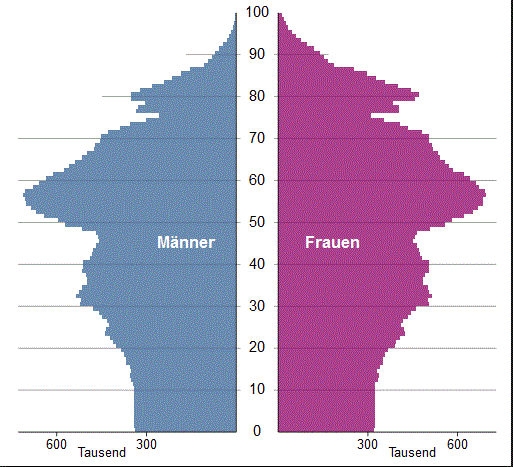
\includegraphics[width=\columnwidth]{image/roman/malefemale.png}
\caption{Gender gap}
\label{fig:malefemale} 
\end{figure}

\subsection{References both academic and commercial tools used}

Tools used in this project: \\
https://public.tableau.com/en-us/s/ \\
Data taken from: \\
https://data.oecd.org/healthstat/suicide-rates.htm \\
https://data.oecd.org/unemp/unemployment-rate.htm \\
https://data.oecd.org/inequality/poverty-rate.htm \\
https://data.oecd.org/gdp/gross-domestic-product-gdp.htm \\
Other resources used: \\
http://www.cs.ubc.ca/~tmm/courses/533-11/resources.html \\

\section{Approach}

\subsection{Description (of our visualization design):}

The approach was to build a tool for end users, so they can discover and get insight into suicide rates. And for us, to practice visualisation techniques from this course. For this reasons we choose a huge dataset containing lots of usable data. OECD website has a lot of public datasets available. We thought of combining suicide data with poverty rates, GDP and unemployment rates to see, if these matches together.
We discussed a lot of ideas, talked about possible solutions and how to implement the course content. Then we build a prototype with many example views. 
Next step was to get feedback and improve the views. We picked the best visualization and refined them. So then we finally came up with a single dashboard.


\subsection{Brief description of the dashboard views:}

The dashboard(Figure \ref{fig:dash}) contains a huge map that is zoom and panable, shows data on the different countries with available information. The heatmap shows the number of suicides, a darker blue indicates a higher suicide rate. 
Top right are the different values shown, each of these 41 in a individual color.
Bottom left is the timeline, a drop down menu can be used to show different data in comparison to the suicide rate(GDB, poverty and unemployment rate). A filters can be applied to the timeline. And then we have this scatter plot showing how this data correlates. On mouse over the users get a little tooltip window showing information.
Multiple elements selected and be filtered.

\begin{figure}[tb]
\centering
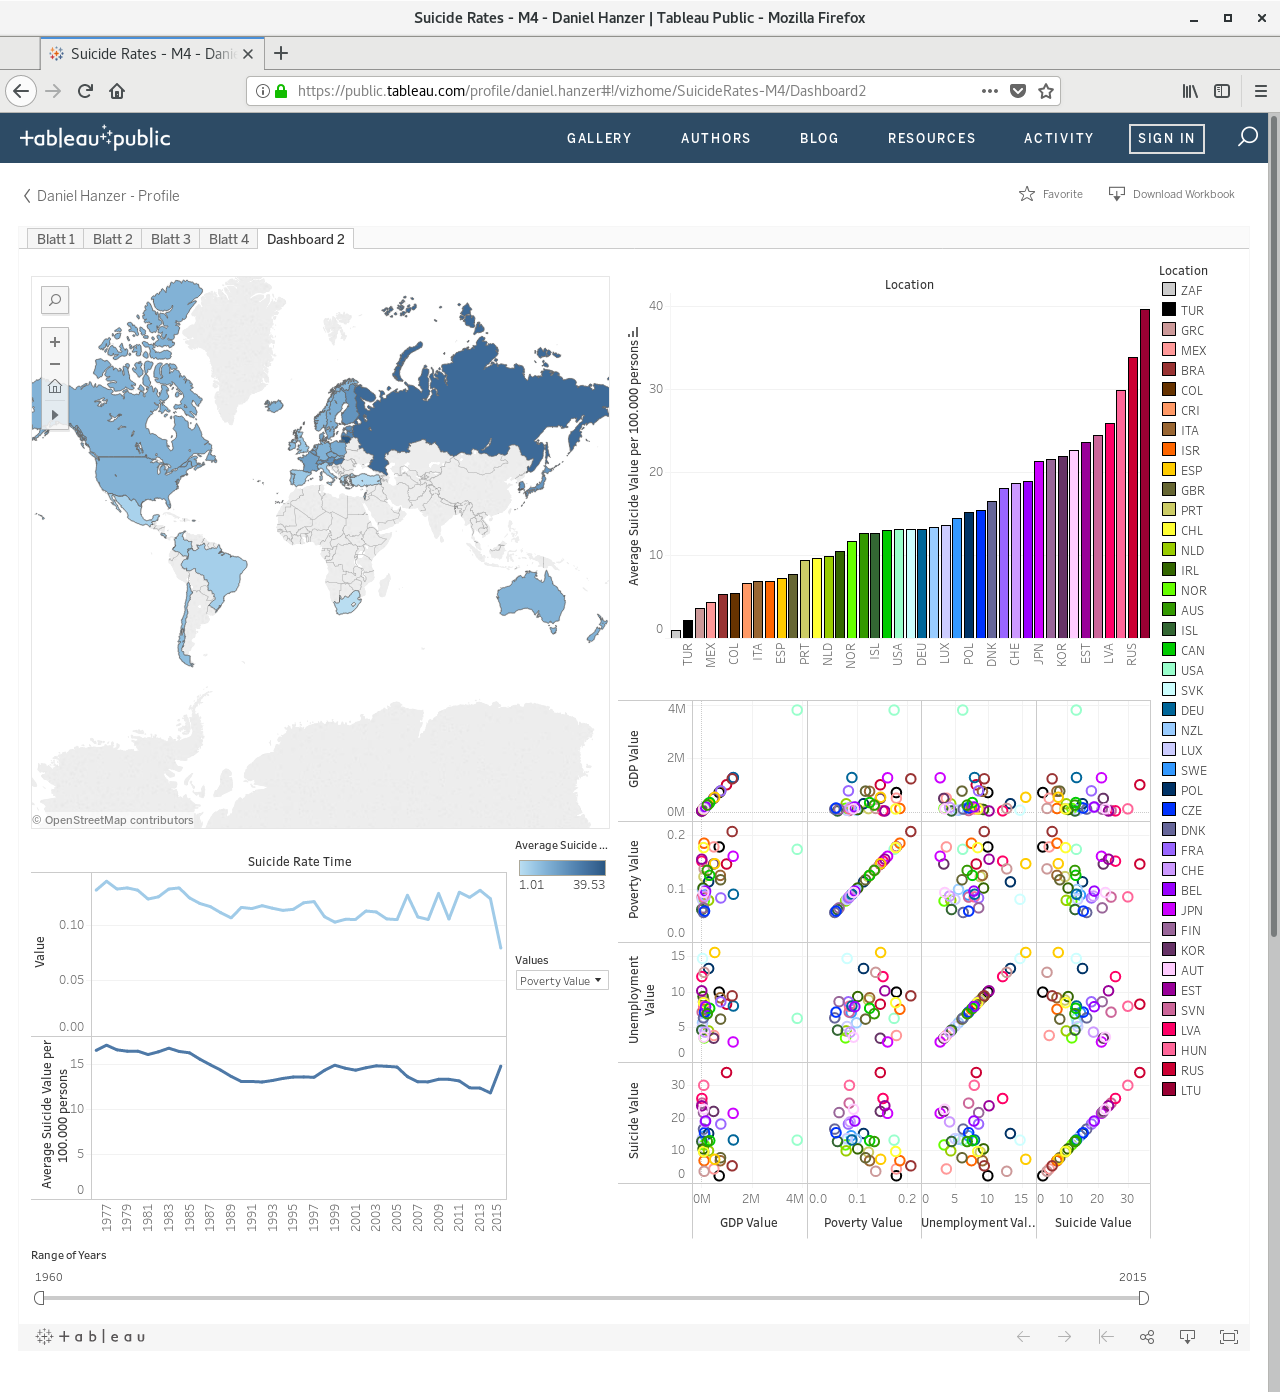
\includegraphics[width=\columnwidth]{image/roman/tableau.png}
\caption{dashboard view}
\label{fig:dash} 
\end{figure}

\section{Implementation}

\subsection{Brief description of the Implementation}

We decided to make use of Tableau after discussing other more technically challenging toolkits like d3 library. Our design study project on mind we have come to think about simplicity, focusing on the usability and interaction possibilities of a proven solution. Previously we worked with Tableau, that's why we decided to use it. On the other hand, there are some limitations that go along with it. 


\subsection{Implementation challenges}

Implementation issues encountered, Public Tableau naturally has some restrictions to what can be accomplished.
The used datasets were fairly huge. Joining the data together often resulted unexpected program behavior. The original datasets were missing some information, so there is no data provided for all countries. In the original data there were different scales used on the data. Some filters were hard to apply, also the selection in the drop down menu.
Creating 41 different colors for the country list was also difficult.

\subsection{Reasons for design choices}
At the beginning we had focused on both, the data and ways to visualize them. The main questioned was, who is the audience. Which end users might want to use this visualization. In which facts they might be interested in? How they gonna use it? So we collected information and feedback and included it in our work.

For this reason one thing we focused on a clear design with high data-ink ratio. There shouldn’t be a distraction from unnecessary chart chunk or from distracting colors. The design is simple, the user interface is easy to use and the charts gives easy to read information an overall good overview.
The feedback we received was altogether pretty good. No one had problems using it, for most of them is seemed very familiar from the start. So this is an good entry point to explore the data further.
On top of that the Functionality-Usability-Aesthetics Pyramide was implemented as well.

\section{Results}

\subsection{Scenarios of use examples}
\begin{itemize}
\item Researching the impact of events on suicide rates

A researcher wants to view the impact on suicide rates in a country of a certain event that happened in 1985. For this, the researcher selects the country in the map view (Figure \ref{fig:resMap}) and selects a appropriate time scale (Figure \ref{fig:resTime}).

In the line chart (Figure \ref{fig:resLine}) a slightly lower suicide rate in Canada in the year 1985 is visible.

\item Researching how much / if economical factors influence the suicide rates in different countries

We select multiple European countries with CTRL + click on the map view as shown in Figure \ref{fig:resMapM}. In the color coded scatter plot matrix (shown in Figure \ref{fig:resScatter}) you can compare the correlation between various economical factors and suicide rates in the selected European countries.

\item Simply comparing suicide rates in different countries

Without selecting anything, per default our visualization shows the suicide rates of all countries (with available data) in a bar chart. As you can see in Figure \ref{fig:resBarChart}, the bar chart features color coding (identical to scatter plot matrix) and a mouse-over hint.

This default view should show the large differences in suicide rates in the various countries and encourage interest to the question "Why is that?". The user can now play around with the other charts and try to find possible explanations in economical factors.

\begin{figure}[tb]
\centering
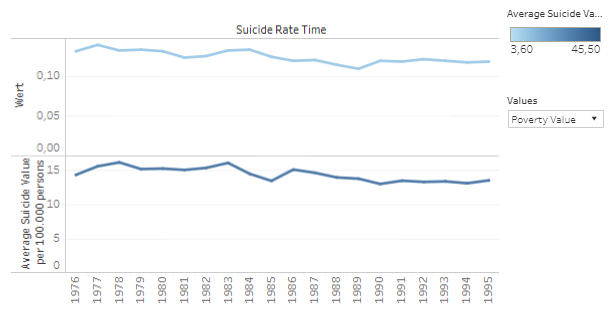
\includegraphics[width=\columnwidth]{image/chris/researcher01.png}
\caption{Line chart showing a dip in the value of suicide rates in Canada of 1985}
\label{fig:resLine} 
\end{figure}

\begin{figure}[tb]
\centering
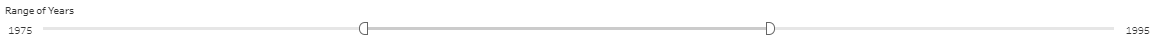
\includegraphics[width=\columnwidth]{image/chris/researcher02.png}
\caption{Selecting a time scale for a more detailed view}
\label{fig:resTime} 
\end{figure}

\begin{figure}[tb]
\centering
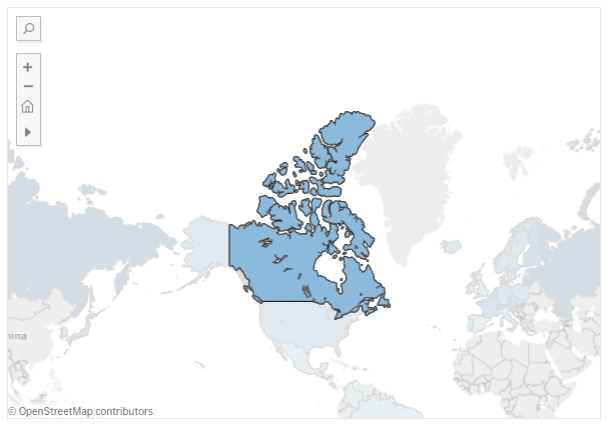
\includegraphics[width=\columnwidth]{image/chris/researcher03.png}
\caption{Map view}
\label{fig:resMap} 
\end{figure}

\begin{figure}[tb]
\centering
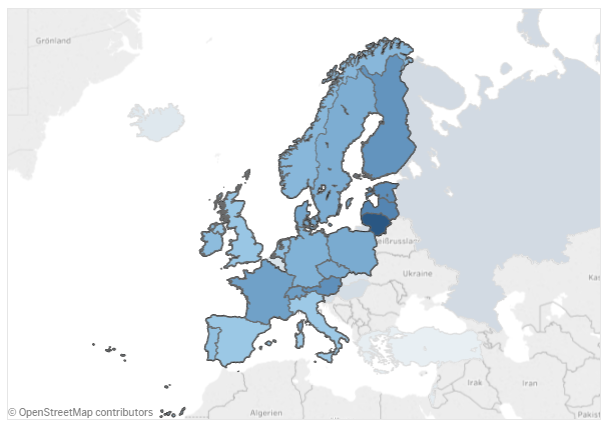
\includegraphics[width=\columnwidth]{image/chris/researcher04.png}
\caption{Multiple selection on map view}
\label{fig:resMapM} 
\end{figure}

\begin{figure}[tb]
\centering
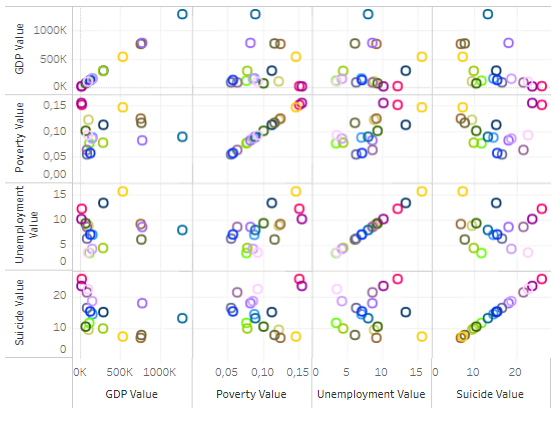
\includegraphics[width=\columnwidth]{image/chris/researcher05.png}
\caption{Scatter plot matrix}
\label{fig:resScatter} 
\end{figure}

\begin{figure}[tb]
\centering
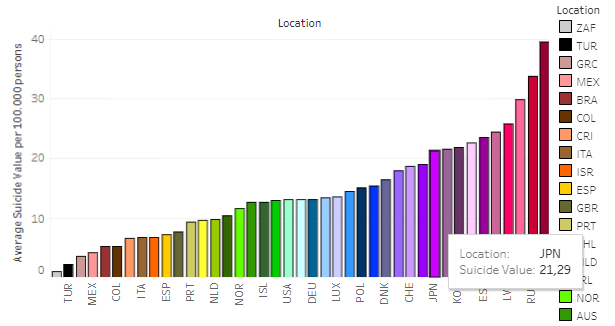
\includegraphics[width=\columnwidth]{image/chris/researcher06.png}
\caption{Default view of bar chart with mouse-over hint}
\label{fig:resBarChart} 
\end{figure}

\end{itemize}

\subsection{Performance of the system}
We designed, tested and improved our visualization to perform well with the intended use case scenarios, including but not limited to the ones detailed in 5.1.

The performance in speed is limited by our visualization tool of choice (Tableau) and the size of the dataset. We discussed limiting the dataset, but that would possibly lower the functionality for a rather small usability gain and could also violate the design principle to show context.

\subsection{Feedback from evaluations}
User feedback was a vital element in the design and improvement of our visualization. We improved the color coding (Figures \ref{fig:resScatter} and \ref{fig:resBarChart}), implemented a scatter plot matrix instead of multiple scatter plots (or scatter plots selectable by a drop-down menu) and made a split line graph (Figure \ref{fig:resLine}) all based on user feedback and evaluations.

With our final visualization the only user complaint remaining is the loading time when selecting multiple countries one after another and initial difficulties to interpret the scatter plot chart.

\subsection{Findings}


\section{Discussion}

\subsection{Strengths and weaknesses of our visualization}

\subparagraph{Strengths}
Every graph is necessary to visualize the intended concepts - no "chart clutter". Our visualization provides a quick overview of the different suicide rates in many OECD nations per default and makes it easy to compare them, which would probably be the most common use case. For a more detailed analysis it provides the necessary tools to find possible correlations to other factors (economical and developmental).

The scatter plot matrix makes it easier, especially for advanced users, to spot correlation between the visualized data on a grand scale - the line chart on a more time based / historical scale. It can be simplified by restricting the number of countries shown.

\subparagraph{(Possible) Weaknesses}
There are only so many factors we could incorporate into our visualization and it is not guaranteed there are correlations between these factors and suicide rates. If we included more it could lead to a too complex visualization and possibly make it even less likely for users to spot correlations as a result.

Selecting countries in the map view leads to loading times. It is not a very significant problem, but if the user wants to select many countries (for example European countries) it becomes annoying pretty fast. We tried to improve the loading times, but it seems to be a problem with tableau and the size of the datasets.

The scatter plot matrix can be slightly difficult to read and interpret correctly because of its high data density. However we are confident this is the best way to visualize possible correlations between the various datasets and suicide rate among all countries and it enables the user to spot correlations on a grand scale in one graph.

It might be difficult for someone to distinguish the countries through the colors. We have tried to spread the color variation as well as to respect the brightness, but seeing up to 41 countries in the visualization can cause readability problems.

If the visualization was filtered by only one country, this leads to that the scatterplot is hardly readable, because the x and y axes adjust automatically depending on the values, if there is only one displayed value, this will show in the upper right corner. Unfortunately, we could not fix the axes, because the values of the different countries are very different and this would mean that the smaller values are all in one spot.

\subsection{Lessons learned}

\begin{itemize}
\item Visualization can be a time consuming process and good time planning is necessary.
\item User feedback is a vital element for visualization. The developers are very likely to overlook possible flaws and shortcomings.
\item Tableau is an easy to use tool if you want your visualization to work and look exactly as the developers intended it to. If you want to do something "non-standard" with this tool, the process can become quite complicated.
\item A good visualization makes it possible to better understand large data sets.
\end{itemize}

\section{Separation of Tasks: Milestone 4}
Christian Rauch:
\begin{itemize}
\item "Results" section
\item "Discussion" section
\item "Separation of Tasks" section
\item LaTeX document setup and coding
\end{itemize}

Daniel Hanzer:
\begin{itemize}
\item Improvements and implementation of feedback in visualization (correct color coding and scatter plot matrix)
\item "Motivation" section
\end{itemize}

Roman Schneglberger:
\begin{itemize}
\item "Related Work" section
\item "Approach" section
\item "Implementation" section
\end{itemize}

\end{document}
